\documentclass{IEEEtran}

\usepackage{graphicx}
\usepackage{amsthm}
\usepackage{amssymb}
\usepackage{amsmath}
\usepackage{algorithm}
\usepackage{algorithmicx}
\usepackage{algpseudocode}
\usepackage{booktabs}
\usepackage{color}

\newcommand{\comment}[1]{}

%\renewcommand{\baselinestretch}{0.95}
%\setlength{\textfloatsep}{0.1cm}
%\setlength{\abovecaptionskip}{0.1cm}

\begin{document}

\title{Differential Privacy on Ranked Similarity Search over Encrypted Cloud Data}
\author{
Shiyu Ji}
\maketitle

\newtheorem{definition}{Definition}
\theoremstyle{definition}
\newtheorem{theorem}{Theorem}
\theoremstyle{plain}
\newtheorem{lemma}{Lemma}
\theoremstyle{plain}
\newtheorem{corollary}{Corollary}
\theoremstyle{plain}

\section{Problem Formulation}
\subsection{The System and Threat Model}
\begin{figure}
\centering
\includegraphics[width=0.4\textwidth]{system_model.eps}
\caption{The architecture of ranked similarity search over encrypted cloud data.}
\label{fig:system_model}
\end{figure}

%\bibliographystyle{./IEEEtran}
%\bibliography{./sim_privacy}
\end{document}
